\begin{frame}
	\frametitle{Motivación}
	
	Don't reinvent the wheel. Create something new and do it faster and better by building on ROS!
	
	\note{https://www.ros.org/blog/why-ros/}
	
	
	\note{https://www.youtube.com/watch?v=bFDfvKctvV8&list=PLRE44FoOoKf7NzWwxt3W2taZ7BiWyfhCp&index=1}
	
	\note{https://www.youtube.com/watch?v=O0729K-7VEY&list=PLNw2RD-1J5YYvFGiMafRD_axHrBUGvuIg&index=1}
	
	\note{https://youtu.be/ZQezxGadsqw}

    \vspace*{1cm}
    \begin{figure}
        
\includegraphics[width=0.5\columnwidth]{images/ros_logo.pdf}
    \end{figure}
	
\end{frame}

\begin{frame}
	\frametitle{¿Qué es ROS?}
	
	ROS (Robot Operating System) es un kit de desarrollo de software de código abierto para aplicaciones de robótica. ROS ofrece una plataforma de software estándar para desarrolladores de todas las industrias que los llevará desde la investigación y la creación de prototipos hasta la implementación y la producción.
	
	\begin{itemize}
		\item Comunidad global
		\item Utilizado en cursos de robótica, investigación e industria
		\item Acorta los tiempos de producción
		\item Multi-dominio: indoor / outdoor, hogareño / industrial, bajo el agua / espacio
		\item Multi-plataforma: Linux, Windows y macOS.
		\item Open-source
		\item Licencia permisiva (Apache 2.0)
		\item Soporte desde la industria
	\end{itemize}
	
	
	\note{https://www.ros.org/blog/why-ros/}
	
	
\end{frame}

\begin{frame}
	\frametitle{¿Qué es ROS?}
    Trabajaremos con la versión Ubuntu LTS más actual, esta siempre viene con una versión de ROS estable.
    \note{ROS 2 distribution released yearly on May 23rd (World Turtle Day).}
	
    \begin{itemize}
    \item Distribución ROS1: Noetic
    \item Distribución actual de ROS2: ver \href{https://docs.ros.org/en/rolling/Releases.html}{https://docs.ros.org/en/rolling/Releases.html}
    \end{itemize}
\end{frame}

\begin{frame}[fragile]
	\frametitle{Instalar ROS}
    \scriptsize
    \begin{itemize}
        \item Seguiremos la guía: \href{https://docs.ros.org/en/<distro>/Tutorials.html}{https://docs.ros.org/en/<distro>/Tutorials.html}
        \item Instalar ROS
        \begin{lstlisting}[style=bash]
sudo apt install ros-<distro>-<package>
        \end{lstlisting}

        \item Sourcear los archivos de setup
        \begin{lstlisting}[style=bash]source /usr/share/gazebo/setup.bash
source /opt/ros/<distro>/setup.bash
        \end{lstlisting}

        \item Agregar el source al .bashrc
        \begin{lstlisting}[style=bash]
echo "source /opt/ros/<distro>/setup.bash" >> ~/.bashrc
        \end{lstlisting}

        \item Chequear las variables de entorno
        \begin{lstlisting}[style=bash]
printenv | grep -i ROS
        \end{lstlisting}

        \item Output:
        \begin{lstlisting}[style=bash]
ROS_VERSION=2
ROS_PYTHON_VERSION=3
ROS_DISTRO=<distro>
        \end{lstlisting}	
        
        \item Chequear el setup de ROS y problemas potenciales (lista de paquetes instalados, versiones, etc)
        
        \begin{lstlisting}[style=bash]
ros2 doctor --report
        \end{lstlisting}
    \end{itemize}
\end{frame}

\begin{frame}[fragile]
	\frametitle{Configuración de entorno de ROS: \lstinline[style=bash]{ROS_DOMAIN_ID}}

\begin{itemize}
    
    \item El middleware predeterminado que utiliza ROS para la comunicación es DDS (\emph{Data Distribution Service}). En DDS, los ID de Dominio permiten que diferentes redes lógicas (cada red lógica tendrá asociado un ID de dominio) compartan una misma red física.
    \item Los nodos en el mismo dominio pueden descubrir y enviarse mensajes libremente, mientras que los nodos en diferentes dominios no pueden.

    \item Todos los nodos utilizan el ID de dominio 0 de forma predeterminada.
    
\begin{lstlisting}[style=bash]
echo "export ROS_DOMAIN_ID=<your_domain_id>" >> ~/.bashrc
\end{lstlisting}
\end{itemize}

\end{frame}

\begin{frame}[fragile]
	\frametitle{Ejemplo: talker y listener}
	
    \begin{itemize}
        \item Primero verifiquemos que esten instalados los ejecutables \lstinline[style=bash]{talker} y \lstinline[style=bash]{listener} de los paquetes \lstinline[style=bash]{demo_nodes_cpp} y \lstinline[style=bash]{demo_nodes_py}
        
        \begin{lstlisting}[style=bash]
ros2 pkg executables
        \end{lstlisting}
        
	    \item En una terminal ejecutar (un talker en c++):
        \begin{lstlisting}[style=bash]
source /opt/ros/<distro>/setup.bash
ros2 run demo_nodes_cpp talker
        \end{lstlisting}

	    \item En otra terminal ejecutar (un listener en python):
        \begin{lstlisting}[style=bash]
source /opt/ros/<distro>/setup.bash
ros2 run demo_nodes_py listener
        \end{lstlisting}
    \end{itemize}

\end{frame}

\begin{frame}[fragile]
    \frametitle{Ejemplo: Turtlesim}
    \scriptsize
    \begin{itemize}

        \item Instalamos el paquete \lstinline[style=bash]{ros-<distro>-turtlesim}
        \begin{lstlisting}[style=bash]
sudo apt install ros-<distro>-turtlesim
        \end{lstlisting}
        \item Verificamos los ejecutables dentro del paquete
        \begin{lstlisting}[style=bash]
ros2 pkg executables turtlesim
        \end{lstlisting}
        \begin{lstlisting}[style=bash]
turtlesim draw_square
turtlesim mimic
turtlesim turtle_teleop_key
turtlesim turtlesim_node
        \end{lstlisting}
        \item Corremos los ejecutables:
        \begin{lstlisting}[style=bash]
ros2 run turtlesim turtlesim_node
        \end{lstlisting}

        \begin{lstlisting}[style=bash]
ros2 run turtlesim turtle_teleop_key
        \end{lstlisting}
        \begin{lstlisting}[style=bash]
ros2 node list
ros2 topic list
ros2 service list
ros2 action list
        \end{lstlisting}
    \end{itemize}    
\end{frame}

\begin{frame}[fragile]
	\frametitle{Ejemplo: Turtlesim (Continuación)}
    
    \begin{itemize}
        \item Abrir \lstinline[style=bash]{rqt}
        \begin{lstlisting}[style=bash]    
rqt
        \end{lstlisting}
        \item Plugins $\rightarrow$ Services $\rightarrow$ Service Caller y spawn una nueva tortuga.
        
        \footnotesize
        \begin{lstlisting}[style=bash]    
ros2 run turtlesim turtle_teleop_key --ros-args --remap turtle1/cmd_vel:=turtle2/cmd_vel
        \end{lstlisting}
    \end{itemize}


\end{frame}

\begin{frame}
    \frametitle{ROS Graph}
    \scriptsize
   	\begin{center}
        \movie[autostart,loop,poster]{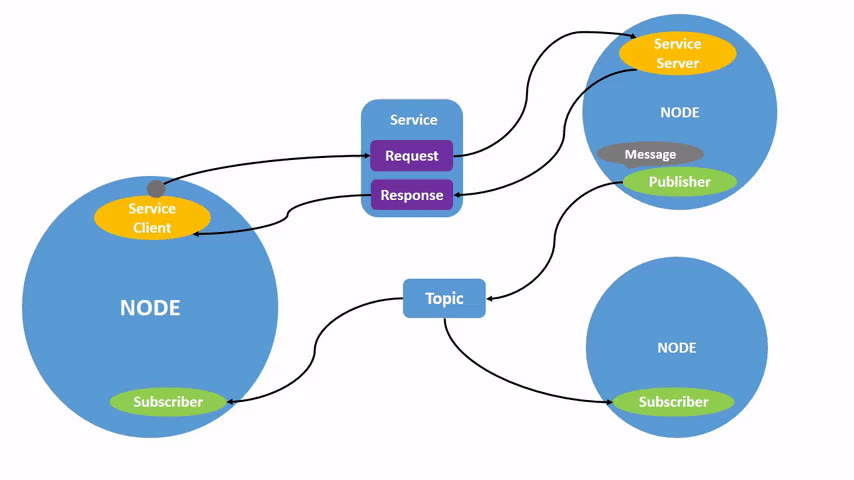
\includegraphics[width=0.5\columnwidth]{images/ros2_nodes_video.jpg}}{videos/ros2_nodes.mp4}
    \end{center}
    
    \begin{itemize}
    \item El grafo de ROS es una red de elementos que procesan datos al mismo tiempo. Abarca todos los ejecutables y las conexiones entre ellos.

    \item Cada nodo en ROS debe ser responsable de un solo propósito de módulo (por ejemplo, un nodo para controlar los motores de las ruedas, un nodo para controlar un telémetro láser, etc.). Cada nodo puede enviar y recibir datos a otros nodos a través de tópicos, servicios, acciones o parámetros.

    \item Un sistema robótico completo se compone de muchos nodos que trabajan en conjunto. En ROS, un único ejecutable (programa C++, programa Python, etc.) puede contener uno o más nodos.
    \end{itemize}
    

\end{frame}

\begin{frame}[fragile]
    \frametitle{Volvamos al Turtlesim para ver otros conceptos}
    
    \begin{itemize}
    

        \item El comando \lstinline[style=bash]{ros2 run} corre un ejecutable desde un paquete.
\begin{lstlisting}[style=bash]    
ros2 run <package_name> <executable_name>
\end{lstlisting}

        \item La \lstinline[style=bash]{ros2 node list} muestra los nombres de todos los nodos en ejecución.

\begin{lstlisting}[style=bash]    
ros2 node list
\end{lstlisting}

        \item Es posible hacer \emph{remapping}, es decir mapear propiedades predeterminadas de un nodo, como nombre de nodo, nombres de tópicos, nombres de servicio, etc., a valores personalizados.
    
\begin{lstlisting}[style=bash]    
ros2 run turtlesim turtlesim_node --ros-args --remap __node:=my_turtle
\end{lstlisting}

        \item Obtener información de un nodo
\begin{lstlisting}[style=bash]    
ros2 node info <node_name>
\end{lstlisting}

    \end{itemize}
\end{frame}

\begin{frame}[fragile]
    \frametitle{Volvamos al Turtlesim para ver otros conceptos (cont.)}
	\footnotesize
	\begin{itemize}
        \item Visualizar los nodos y la comunicación entre los mismos:
\begin{lstlisting}[style=bash]  
rqt_graph
\end{lstlisting}

        \item Devuelve la misma lista de tópicos, esta vez con el tipo de tema entre paréntesis:
\begin{lstlisting}[style=bash]  
ros2 topic list -t
\end{lstlisting}
    
        \item Ver los datos publicados en un tópico:
\begin{lstlisting}[style=bash]  
ros2 topic echo <topic_name>
\end{lstlisting}
    
        Ejemplo:
\begin{lstlisting}[style=bash]  
ros2 topic echo /turtle1/cmd_vel
\end{lstlisting}
    
        \item Obtener información acerca de los publicadores y subscriptores de un tópico:
\begin{lstlisting}[style=bash]  
ros2 topic info
\end{lstlisting}
    
        \item Obtener detalles sobre un tipo de mensaje:
\begin{lstlisting}[style=bash]  
ros2 interface show <msg type>
\end{lstlisting}    

        Ejemplo:
\begin{lstlisting}[style=bash]  
ros2 interface show geometry_msgs/msg/Twist
\end{lstlisting}

    \end{itemize}

\end{frame}

\begin{frame}[fragile]
	\frametitle{Volvamos al Turtlesim para ver otros conceptos (cont.)}
    \begin{itemize}
        \item Publicar mensajes utilizando la línea de comandos:

\begin{lstlisting}[style=bash]  
ros2 topic pub <topic_name> <msg_type> '<args>'
\end{lstlisting}    

Ejemplo:

\begin{lstlisting}[style=bash,basicstyle=\tiny]  
ros2 topic pub --rate 1 /turtle1/cmd_vel geometry_msgs/msg/Twist "{linear: {x: 2.0, y: 0.0, z: 0.0}, angular: {x: 0.0, y: 0.0, z: 1.8}}"
\end{lstlisting}    

\item Saber la prefuencia en que se publica un mensaje

\begin{lstlisting}[style=bash]  
ros2 topic hz <topic_name>
\end{lstlisting}
    \end{itemize}
\end{frame}

\begin{frame}[fragile]
	\frametitle{Archivos launch}
	
    \begin{itemize}
        \item A medida que se crean sistemas más complejos con más y más nodos ejecutándose simultáneamente, abrir terminales y volver a ingresar los detalles de configuración se vuelve tedioso.

        \item Los archivos \emph{launch} permiten iniciar y configurar varios ejecutables que contienen nodos ROS 2 de manera simultáneamente.

        \item Ejecutar un solo archivo launch con el comando \lstinline[style=bash]{ros2 launch} iniciará todo su sistema, todos los nodos y sus configuraciones, a la vez.

Correr un archivo launch
\begin{lstlisting}[style=bash] 
ros2 launch <package_name> <launch_file_name> <launch_arguments>
\end{lstlisting}

Ejemplo:
\begin{lstlisting}[style=bash] 
ros2 launch turtlesim multisim.launch.py
\end{lstlisting}

    \end{itemize}
\end{frame}


\begin{frame}[fragile]
    \frametitle{Crear workspace}
    
    \begin{itemize}
        \item Crear workspace
        \begin{lstlisting}[style=bash] 
mkdir -p ~/dev_ws/src
cd ~/dev\_ws/src
        \end{lstlisting}
        
        \item Un \emph{workspace} es un directorio que contiene paquetes de ROS 2.
        \item Antes de usar ROS 2, es necesario obtener su espacio de trabajo de instalación de ROS 2 en la terminal en la que planea trabajar. Esto hace que los paquetes de ROS 2 estén disponibles para que los use en esa terminal. Para esto hacemos:
        
\begin{lstlisting}[style=bash] 
source /opt/ros/<distro>/setup.bash
\end{lstlisting}
        


\item Agregar un paquete de ejemplo al workspace (dentro de \lstinline[style=bash]{~/dev\_ws/src})
\begin{lstlisting}[style=bash] 
git clone https://github.com/ros2/examples examples -b <distro>
\end{lstlisting}

\begin{lstlisting}[style=bash] 
git clone https://github.com/ros/ros\_tutorials.git -b <distro>-devel
\end{lstlisting}
    \end{itemize}
\end{frame}


\begin{frame}[fragile]
	\frametitle{Compilar el workspace}
\begin{itemize}
    \item Instalar colcon
\begin{lstlisting}[style=bash] 
sudo apt install python3-colcon-common-extensions
\end{lstlisting}

    \item En la raíz del workspace, ejecutar
\begin{lstlisting}[style=bash] 
colcon build --symlink-install
\end{lstlisting}

	El flag \lstinline[style=bash]{--symlink-install} permite usar enlaces simbólicos, en lugar de copiar archivos a las carpetas de ROS2 durante la instalación, siempre que sea posible. Cada paquete en ROS2 debe instalarse y todos los archivos utilizados por los nodos deben copiarse en las carpetas de instalación.
	
	\item El build genera los directorios: \lstinline[style=bash]{build}, \lstinline[style=bash]{install} y \lstinline[style=bash]{log}.
\end{itemize}
\end{frame}

\begin{frame}[fragile]
	\frametitle{Compilar el workspace}
	\begin{itemize}

	   \item Cuando \lstinline[style=bash]{colcon} haya completado el build, la salida estará en el directorio  \lstinline[style=bash]{install}.
       \item \lstinline[style=bash]{colcon} genera archivos \lstinline[style=bash]{bash/bat} en el directorio \lstinline[style=bash]{install} para ayudar a configurar el entorno. Estos archivos agregarán todos los elementos requeridos a su ruta y rutas de biblioteca, así como también proporcionarán cualquier comando bash o shell exportado por los paquetes.

        \item Ejemplo de uso: (no olvidar \lstinline[style=bash]{source install/setup.bash})
\begin{lstlisting}[style=bash] 
ros2 run examples_rclcpp_minimal_subscriber subscriber_member_function
\end{lstlisting}

\begin{lstlisting}[style=bash] 
ros2 run examples_rclcpp_minimal_publisher publisher_member_function
\end{lstlisting}
\item El comando \lstinline[style=bash]{colcon_cd} le permite cambiar rápidamente el directorio de trabajo actual al de un paquete.
    \end{itemize}

\end{frame}

\begin{frame}[fragile]
	\frametitle{Creando un paquete en ROS2}
    
    \begin{itemize}
        \item Un paquete puede considerarse un contenedor para código ROS 2. 

        \item La creación de paquetes en ROS 2 utiliza \lstinline[style=bash]{ament} como sistema de compilación y \lstinline[style=bash]{colcon} como herramienta de compilación.
        
        \item Hay paquetes que utilizan CMake, y otros Python:
        \begin{itemize}
            \item CMake:
            \begin{itemize}
            	\item \lstinline[style=bash]{package.xml} contiene meta información del paquete
            
            	\item \lstinline[style=bash]{CMakeLists.txt} describe cómo compilar el código dentro del paquete
            \end{itemize}
    
            \item Python:
            \begin{itemize}
                \item \lstinline[style=bash]{package.xml} contiene meta información del paquete
                
                \item \lstinline[style=bash]{setup.py} contiene instrucciones para de cómo instalar el paquete
                
                \item \lstinline[style=bash]{setup.cfg} es requerido cuando un paquete tiene ejecutables, así ROS 2 puede encontrarlos
                
                \item \lstinline[style=bash]{/<package_name>} un directorio con el mismo nombre del paquete. Este es usado por ROS 2 para encontrar el paquete, contiene el \lstinline[style=bash]{__init__.py}
            \end{itemize}
        \end{itemize}
    \end{itemize}	
\end{frame}

\begin{frame}[fragile]
	\frametitle{Creando un paquete en ROS2}
    \begin{itemize}
        \item Crear un paquete:
        \begin{lstlisting}[style=bash] 
ros2 pkg create test_pkg --build-type ament_cmake
        \end{lstlisting}

        \item El argumento opcional \lstinline[style=bash]{--node-name} permite crear un ejecutable con un nombre dado en el paquete.
        \begin{lstlisting}[style=bash] 
ros2 pkg create test_pkg --build-type ament_cmake --node-name <node_name> <package_name>
        \end{lstlisting}
    \end{itemize}	
\end{frame}


\begin{frame}[fragile]
	\frametitle{Ejemplo: creemos un paquete que contenga Publicador y Subscriptor}
    
    \begin{columns}
        \begin{column}{0.5\textwidth}
            \lstinputlisting[style=cpp,basicstyle=\tiny,firstline=1,lastline=23]{src/publisher_member_function.cpp}
        \end{column}
        \begin{column}{0.5\textwidth}
            \lstinputlisting[style=cpp,basicstyle=\tiny,firstline=25,lastline=44]{src/publisher_member_function.cpp}
        \end{column}
    \end{columns}
	
\begin{lstlisting}[style=bash,basicstyle=\footnotesize] 
ros2 run cpp_pubsub talker
\end{lstlisting}
\begin{lstlisting}[style=bash,basicstyle=\footnotesize] 
ros2 run cpp_pubsub listener
\end{lstlisting}
	
\end{frame}

\begin{frame}[fragile]
    \frametitle{Ejemplo: creemos un paquete que contenga Publicador y Subscriptor}
    
    \begin{columns}
        \begin{column}{0.5\textwidth}
            \lstinputlisting[style=cpp,basicstyle=\scriptsize,firstline=1,lastline=15]{src/subscriber_member_function.cpp}
        \end{column}
        \begin{column}{0.5\textwidth}
            \lstinputlisting[style=cpp,basicstyle=\scriptsize,firstline=16,lastline=31]{src/subscriber_member_function.cpp}
        \end{column}
    \end{columns}
    
\end{frame}

\begin{frame}[fragile]
    \frametitle{Ejemplo: creemos un paquete que contenga Publicador y Subscriptor}
    
    \begin{columns}
        \begin{column}{0.5\textwidth}
            \lstinputlisting[style=cmake,basicstyle=\scriptsize,firstline=1,lastline=15]{src/CMakeLists.txt}
        \end{column}
        \begin{column}{0.5\textwidth}
            \lstinputlisting[style=cmake,basicstyle=\scriptsize,firstline=16,lastline=28]{src/CMakeLists.txt}
        \end{column}
    \end{columns}
    
    \begin{lstlisting}[style=bash] 
ros2 run cpp_pubsub talker
    \end{lstlisting}

    \begin{lstlisting}[style=bash] 
ros2 run cpp_pubsub listener
    \end{lstlisting}
\end{frame}


\begin{frame}[fragile]
    \frametitle{Rosbags (\lstinline[style=bash]{ros2 bag})}
    \begin{itemize}
        \item \lstinline[style=bash]{ros2 bag} es una herramienta de línea de comandos para grabar datos publicados sobre tópicos en su sistema.
        \item Acumula los datos transmitidos sobre cualquier número de tópicos y los guarda en una base de datos. 
        \item Luego, puede reproducir los datos para reproducir los resultados de sus pruebas y experimentos.
        \item Grabar tópicos también es una excelente manera de compartir el trabajo y permitir que otros lo reproduzcan.
        
        \begin{lstlisting}[style=bash] 
ros2 bag record <topic_name>
ros2 bag info <bag_file_name>
ros2 bag play <bag_file_name>
ros2 bag compress <bag_file_name>
ros2 bag decompress <bag_file_name>
...
        \end{lstlisting}
    \end{itemize}
\end{frame}


\begin{frame}[fragile]
	\frametitle{Ejemplo completo: Navegación con Turtlebot3}

    \footnotesize
    \begin{itemize}


        \item Ver la Guía: \url{https://navigation.ros.org}
    
        \item Instalar los paquetes de Nav2 
        
        \begin{lstlisting}[style=bash] 
sudo apt install ros-<ros2-distro>-navigation2 ros-<ros2-distro>-nav2-bringup
        \end{lstlisting}
    
        \item Instalar los paquetes de Turtlebot 3
        
        \begin{lstlisting}[style=bash] 
sudo apt install ros-<ros2-distro>-turtlebot3*
        \end{lstlisting}
    
        \item Setear las variables de entorno y sourcear Gazebo (recuerde agregar estas líneas a \lstinline[style=bash]{.bashrc}):
        
        \begin{lstlisting}[style=bash] 
export TURTLEBOT3_MODEL=waffle
export GAZEBO_MODEL_PATH=$GAZEBO_MODEL_PATH:/opt/ros/<ros2-distro>/share/turtlebot3_gazebo/models
source /usr/share/gazebo/setup.bash
        \end{lstlisting}
    
        \item Lanzar la simulación. El parámetro \lstinline[style=bash]{headless:=False} permite visualizar el simulador Gazebo.
        
        \begin{lstlisting}[style=bash] 
ros2 launch nav2_bringup tb3_simulation_launch.py headless:=False
        \end{lstlisting}
     
    \end{itemize}
    \tiny
    \url{https://ros2-industrial-workshop.readthedocs.io/en/latest/\_source/navigation/ROS2-Navigation.html}
        
    \url{https://docs.ros.org/en/<distro>/Tutorials/Advanced/Simulators/Ignition.html}
        
    \url{https://navigation.ros.org/index.html}

\end{frame}


\begin{frame}[fragile]
    \frametitle{Ejemplo completo: Navegación con Turtlebot3}
    
    \begin{center}
        \movie[autostart,loop,poster]{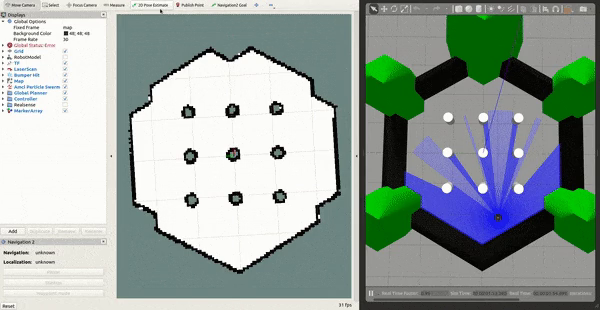
\includegraphics[width=\columnwidth]{images/turtlebot_navigation_video.png}}{videos/turtlebot_navigation.avi}
    \end{center}
    
\end{frame}

\begin{frame}[fragile]
    \frametitle{Sistemas de coordenadas para plataformas Móviles}
    \scriptsize
    \begin{center}
        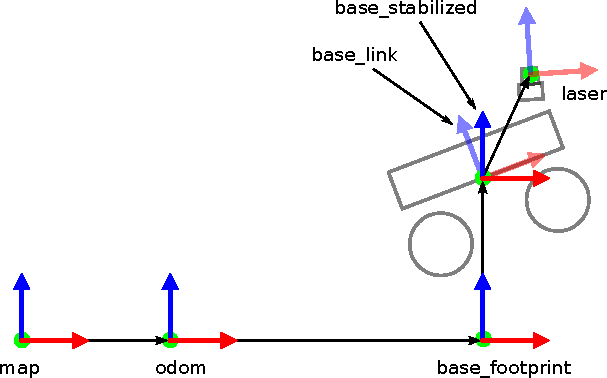
\includegraphics[width=0.3\columnwidth]{images/ros_coordinate_systems.pdf}
    \end{center}
    
    \begin{itemize}
        \item El marco de coordenadas llamado \lstinline[style=bash]{/base_link} está rígidamente unido a la base del robot móvil. El \lstinline[style=bash]{/base_link} es el marco de referencia del robot.
        
        \item El marco \lstinline[style=bash]{/odom} contiene la pose del robot en el mundo según lo informado por algún sensor de odometría (Ej: odometría de ruedas, Visual-Inertial Odometry, etc). La pose del robot en el marco de coordenadas \lstinline[style=bash]{/odom} es continua; sin embargo, debido a errores en la odometría, el error se acumula con el tiempo.
        
        \item Para corregir la desviación de los sensores odométricos, algunos métodos de localización introducen una transformación entre \lstinline[style=bash]{/map} $\rightarrow$ \lstinline[style=bash]{/odom}. Esta transformación es la corrección que se ha calculado en función de la entrada de sensores, como LiDAR o GNSS. La pose del robot en \lstinline[style=bash]{/map} no es continua (puede saltar en varios intervalos de tiempo) porque los métodos de localización que dan este tipo de pose normalmente realizan correcciones a una frecuencia más baja.
        
        \item Si el sensor de odometría y el GNSS son perfectos, la transformación \lstinline[style=bash]{/map} mapa $\rightarrow$ \lstinline[style=bash]{/odom} tf será la identidad.
        
        
    \end{itemize}
    
\end{frame}



\begin{frame}[fragile]
    \frametitle{Estándares/convenciones de ROS: REP (\emph{ROS Enhancement Proposal})}

    \begin{itemize}
        \item REP-103: \emph{Standard Units of Measure and Coordinate Conventions} \url{https://www.ros.org/reps/rep-0103.html}
        
        \item REP-105: \emph{Coordinate Frames for Mobile Platforms} \url{https://ros.org/reps/rep-0105.html#coordinate-frames}
    \end{itemize}
    
\end{frame}

\begin{frame}
	\frametitle{TF: transformaciones en ROS}
	
	\footnotesize
    
    \note{slides de tf2 https://ethz.ch/content/dam/ethz/special-interest/mavt/robotics-n-intelligent-systems/rsl-dam/ROS2021/lec3/ROS\%20Course\%20Slides\%20Course\%203.pdf}
    
    \begin{columns}
		\begin{column}{0.5\textwidth}
			\begin{itemize}
			\item Herramienta para seguir los marcos de coordenada a través del tiempo
			\item Mantiene las relaciones entre los marcos de coordenadas en una estructura de árbol buffereado en el tiempo
			\item Permite transformar puntos, vectores, etc entre marcos de coordenadas para un determinado tiempo
			\item Implementado como un modelo publicador/subscriptor en los tópicos /tf y /tf\_static
			\end{itemize}
		
			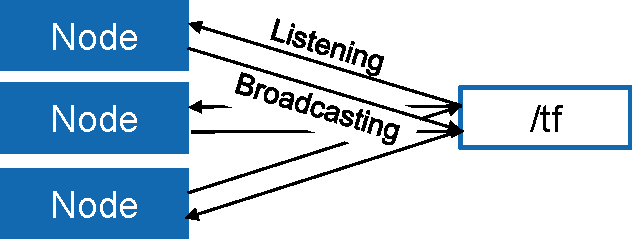
\includegraphics[width=\columnwidth]{images/tf2_broadcaster_listener.pdf}
		\end{column}
		\begin{column}{0.5\textwidth}
			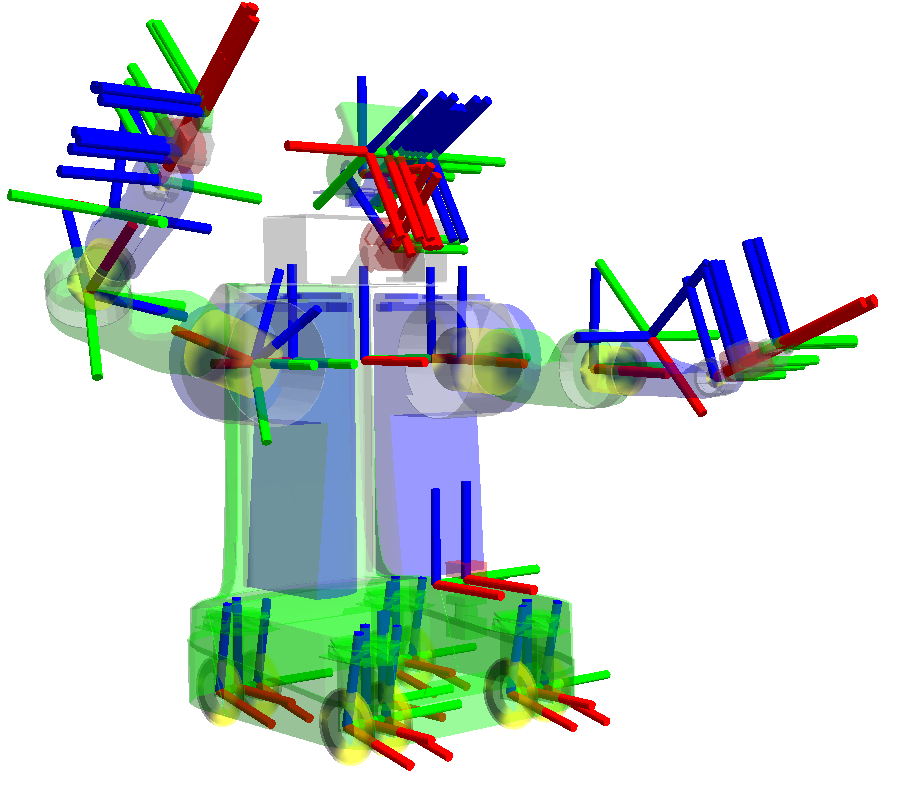
\includegraphics[width=\columnwidth]{images/tf2_tree_robot.png}
		\end{column}
	\end{columns}

\end{frame}

\begin{frame}[fragile]
    \frametitle{TF: transformaciones en ROS}
    \scriptsize
        \begin{columns}
    	\begin{column}{0.5\textwidth}
		    \begin{itemize}
				\item TF listeners usan un buffer para escuchar las transformaciones broadcasteadas
				\item Se puede consultar una transformación específica al árbol de transformaciones
                \item El tipo de mensaje de tf2 (\lstinline[style=bash]{tf2_msgs/TFMessage.msg})
                \begin{lstlisting}[style=bash] 
geometry_msgs/TransformStamped[] transforms
                \end{lstlisting}
                \item El tipo de mensaje \lstinline[style=bash]{geometry_msgs/TransformStamped}
                \begin{lstlisting}[style=bash] 
std_msgs/Header header
uint32 seqtime stamp
string frame_id
string child_frame_id
geometry_msgs/Transform transform
                \end{lstlisting}
                \item El tipo de mensaje \lstinline[style=bash]{geometry_msgs/Transform}
                \begin{lstlisting}[style=bash] 
geometry_msgs/Vector3 translation
geometry_msgs/Quaternion rotation
                \end{lstlisting}
			\end{itemize}
    	\end{column}
    	\begin{column}{0.5\textwidth}
    		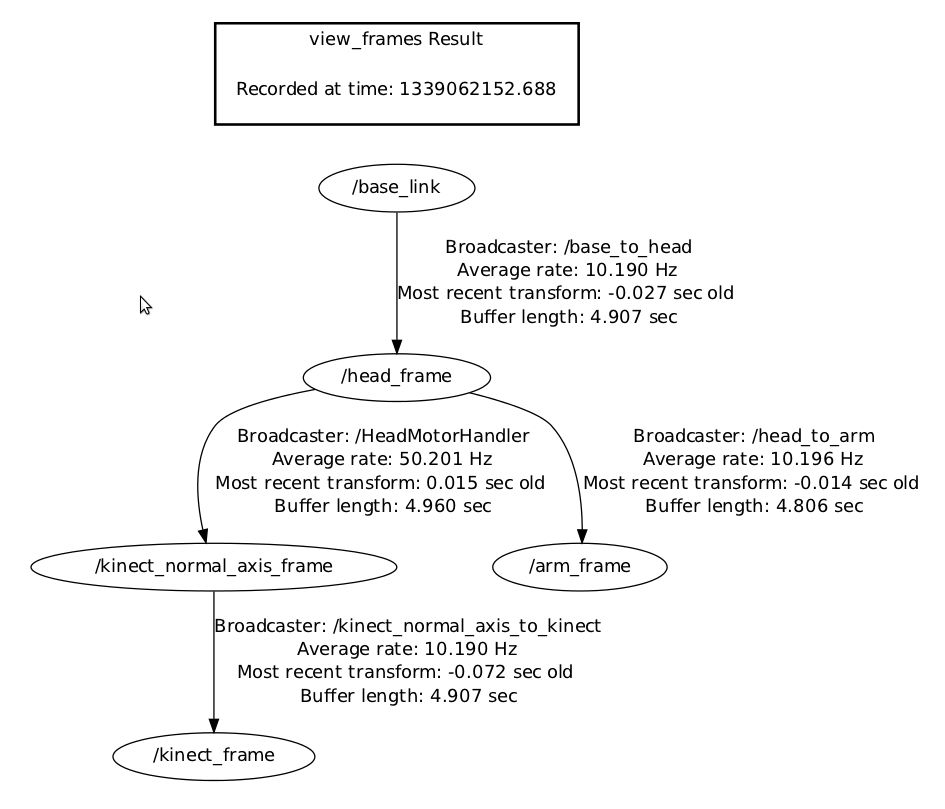
\includegraphics[width=\columnwidth]{images/tf2_tree_graph.png}
    	\end{column}
    \end{columns}
\end{frame}

\begin{frame}[fragile]
    \frametitle{TF: transformaciones en ROS}
    
    \begin{itemize}
        \item Visualizar el árbol de transformaciones:
        \begin{lstlisting}[style=bash] 
ros2 run tf2_tools view_frames
        \end{lstlisting}

        \item Imprimir información a cerca de la transformación entre dos marcos de coordenadas:
        \begin{lstlisting}[style=bash] 
ros2 run tf2_ros tf2_echo [reference_frame] [target_frame]
        \end{lstlisting}
    \end{itemize}

\end{frame}

\begin{frame}
	\frametitle{Visualizar transformaciones en RViz (\lstinline[style=bash]{rviz2})}
	
   	\begin{figure}[!h]
		\centering
			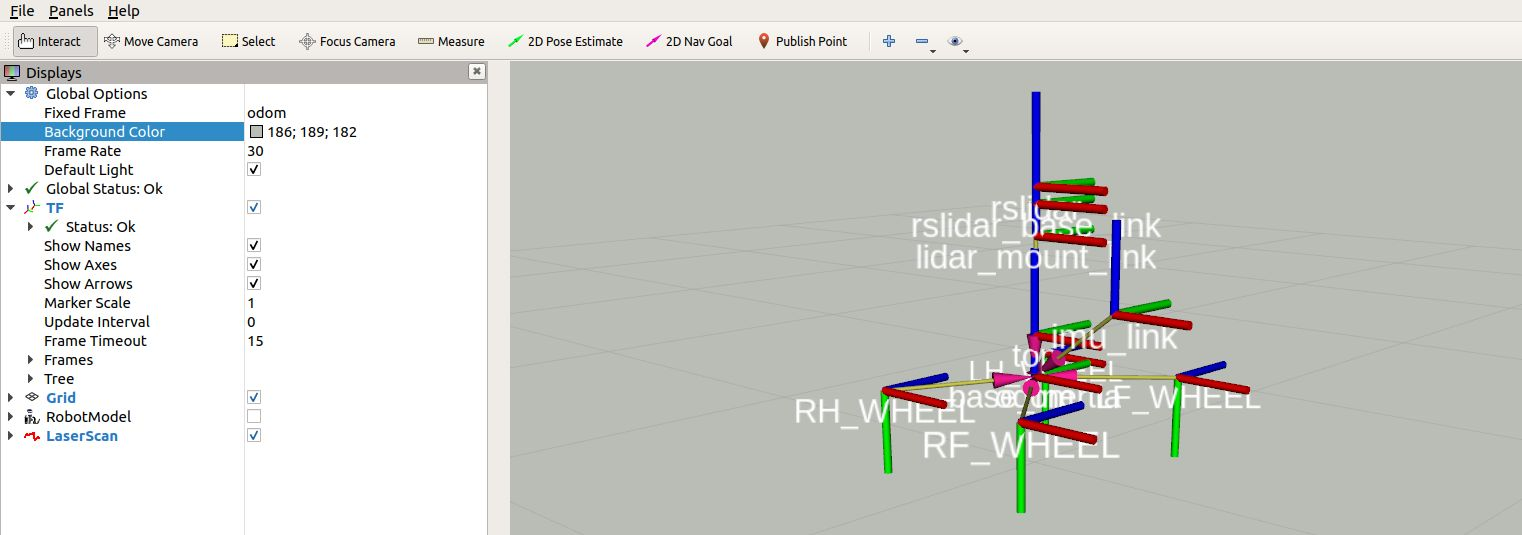
\includegraphics[width=\columnwidth]{images/tf2_tree_rviz.png}
	\end{figure}
	
\end{frame}

\begin{frame}
	\frametitle{Visualizar transformaciones en RViz (\lstinline[style=bash]{rviz2})}
	\begin{figure}[!h]
		\centering
		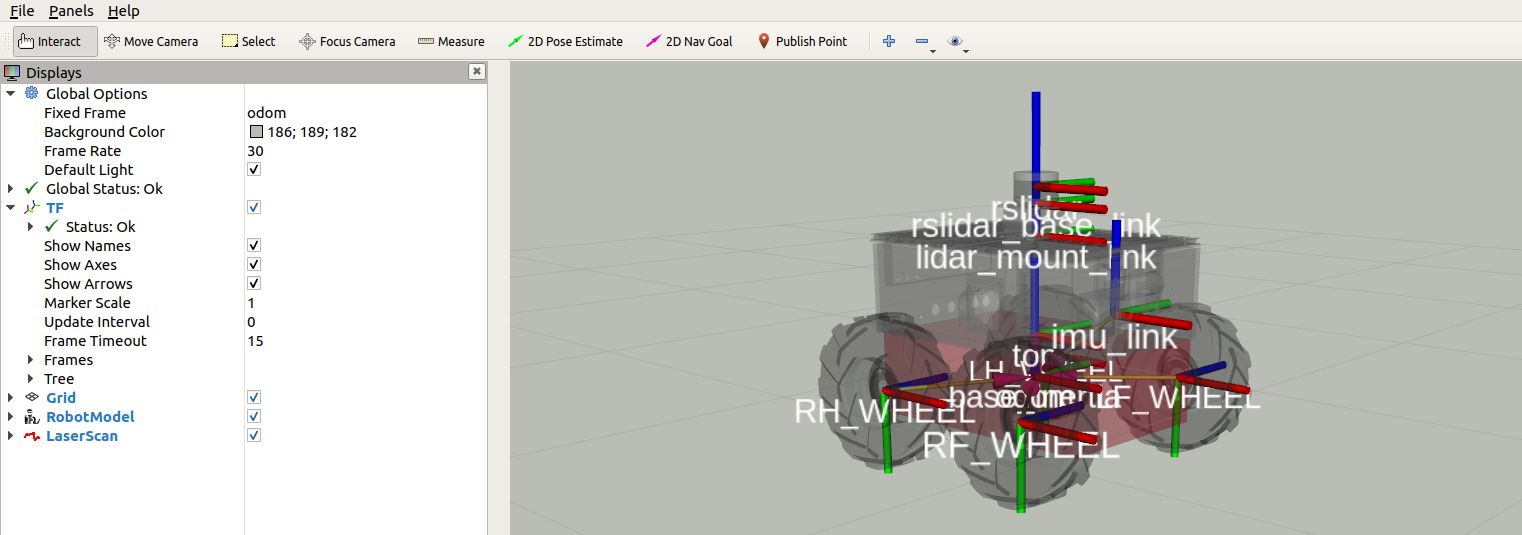
\includegraphics[width=\columnwidth]{images/tf2_tree_robot_rviz.png}
	\end{figure}
	
\end{frame}

\begin{frame}[fragile]
	\frametitle{Ejemplo: TF2 con turtles}
    \scriptsize
	\begin{itemize}
        \item Tutorial: \url{https://docs.ros.org/en/<distro>/Tutorials/Intermediate/Tf2/Introduction-To-Tf2.html}
        \item Instalación
        \begin{lstlisting}[style=bash] 
sudo apt-get install ros-<distro>-turtle-tf2-py ros-<distro>-tf2-tools ros-<distro>-tf-transformations
        \end{lstlisting}
        
        \item En una terminal, lanzar el launch \lstinline[style=bash]{turtle_tf2_demo.launch.py}
        
        \begin{lstlisting}[style=bash] 
ros2 launch turtle_tf2_py turtle_tf2_demo.launch.py
        \end{lstlisting}
        
        \item En otra terminal, ejecutar \lstinline[style=bash]{turtle_teleop_key}
        
        \begin{lstlisting}[style=bash] 
ros2 run turtlesim turtle_teleop_key
        \end{lstlisting}
        
        \item Visualizar el árbol de transformaciones:
        
        \begin{lstlisting}[style=bash] 
ros2 run tf2_tools view_frames
        \end{lstlisting}
        
        \item \lstinline[style=bash]{tf2_echo} informa la transformación entre dos cuadros cualesquiera transmitidos a través de ROS.
        
        \begin{lstlisting}[style=bash] 
ros2 run tf2_ros tf2_echo [source_frame] [target_frame]
        \end{lstlisting}

        \begin{lstlisting}[style=bash] 
ros2 run tf2_ros tf2_echo turtle2 turtle1
        \end{lstlisting}
        
        \item Visualizar en rviz2
        
        \begin{lstlisting}[style=bash] 
ros2 run rviz2 rviz2 -d $(ros2 pkg prefix --share turtle_tf2_py)/rviz/turtle_rviz.rviz
        \end{lstlisting}
        
    \end{itemize}
\end{frame}

\begin{frame}
	\frametitle{Unified Robot description Format (URDF)}
 	\begin{columns}
		\begin{column}{0.5\textwidth}
			\begin{itemize}
				\item Se define en un archivo XML la representación de un modelo del robot
				\begin{itemize}
					\item Descripción de la Cinemática y Dinámica del robot
					\item Representación Visual
					\item Modelo de colisión
				\end{itemize}
				\item La generación del archivo URDF puede ser a través de un script en XACRO
			\end{itemize}
		\end{column}
		\begin{column}{0.5\textwidth}
			\begin{figure}[!h]
			\centering
			\subfloat[Modelo Visual]
			{
				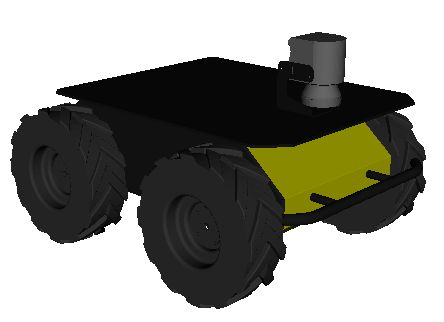
\includegraphics[width=0.4\columnwidth]{images/urdf_visual_model.png}
			}
			\subfloat[Modelo de colisión]
			{
				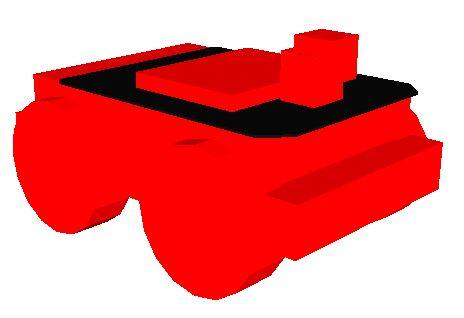
\includegraphics[width=0.4\columnwidth]{images/urdf_collision_model.png}
			}
			\end{figure}
		\end{column}
	\end{columns}
	
\end{frame}

\begin{frame}
	\frametitle{Unified Robot description Format (URDF)}
	
	\begin{itemize}
		\item La descripción consiste en un conjunto de elementos links y un conjunto de elementos joints
		\item Los joints conectan los links entre sí
	\end{itemize}
	
	\begin{figure}[!h]
		\centering
		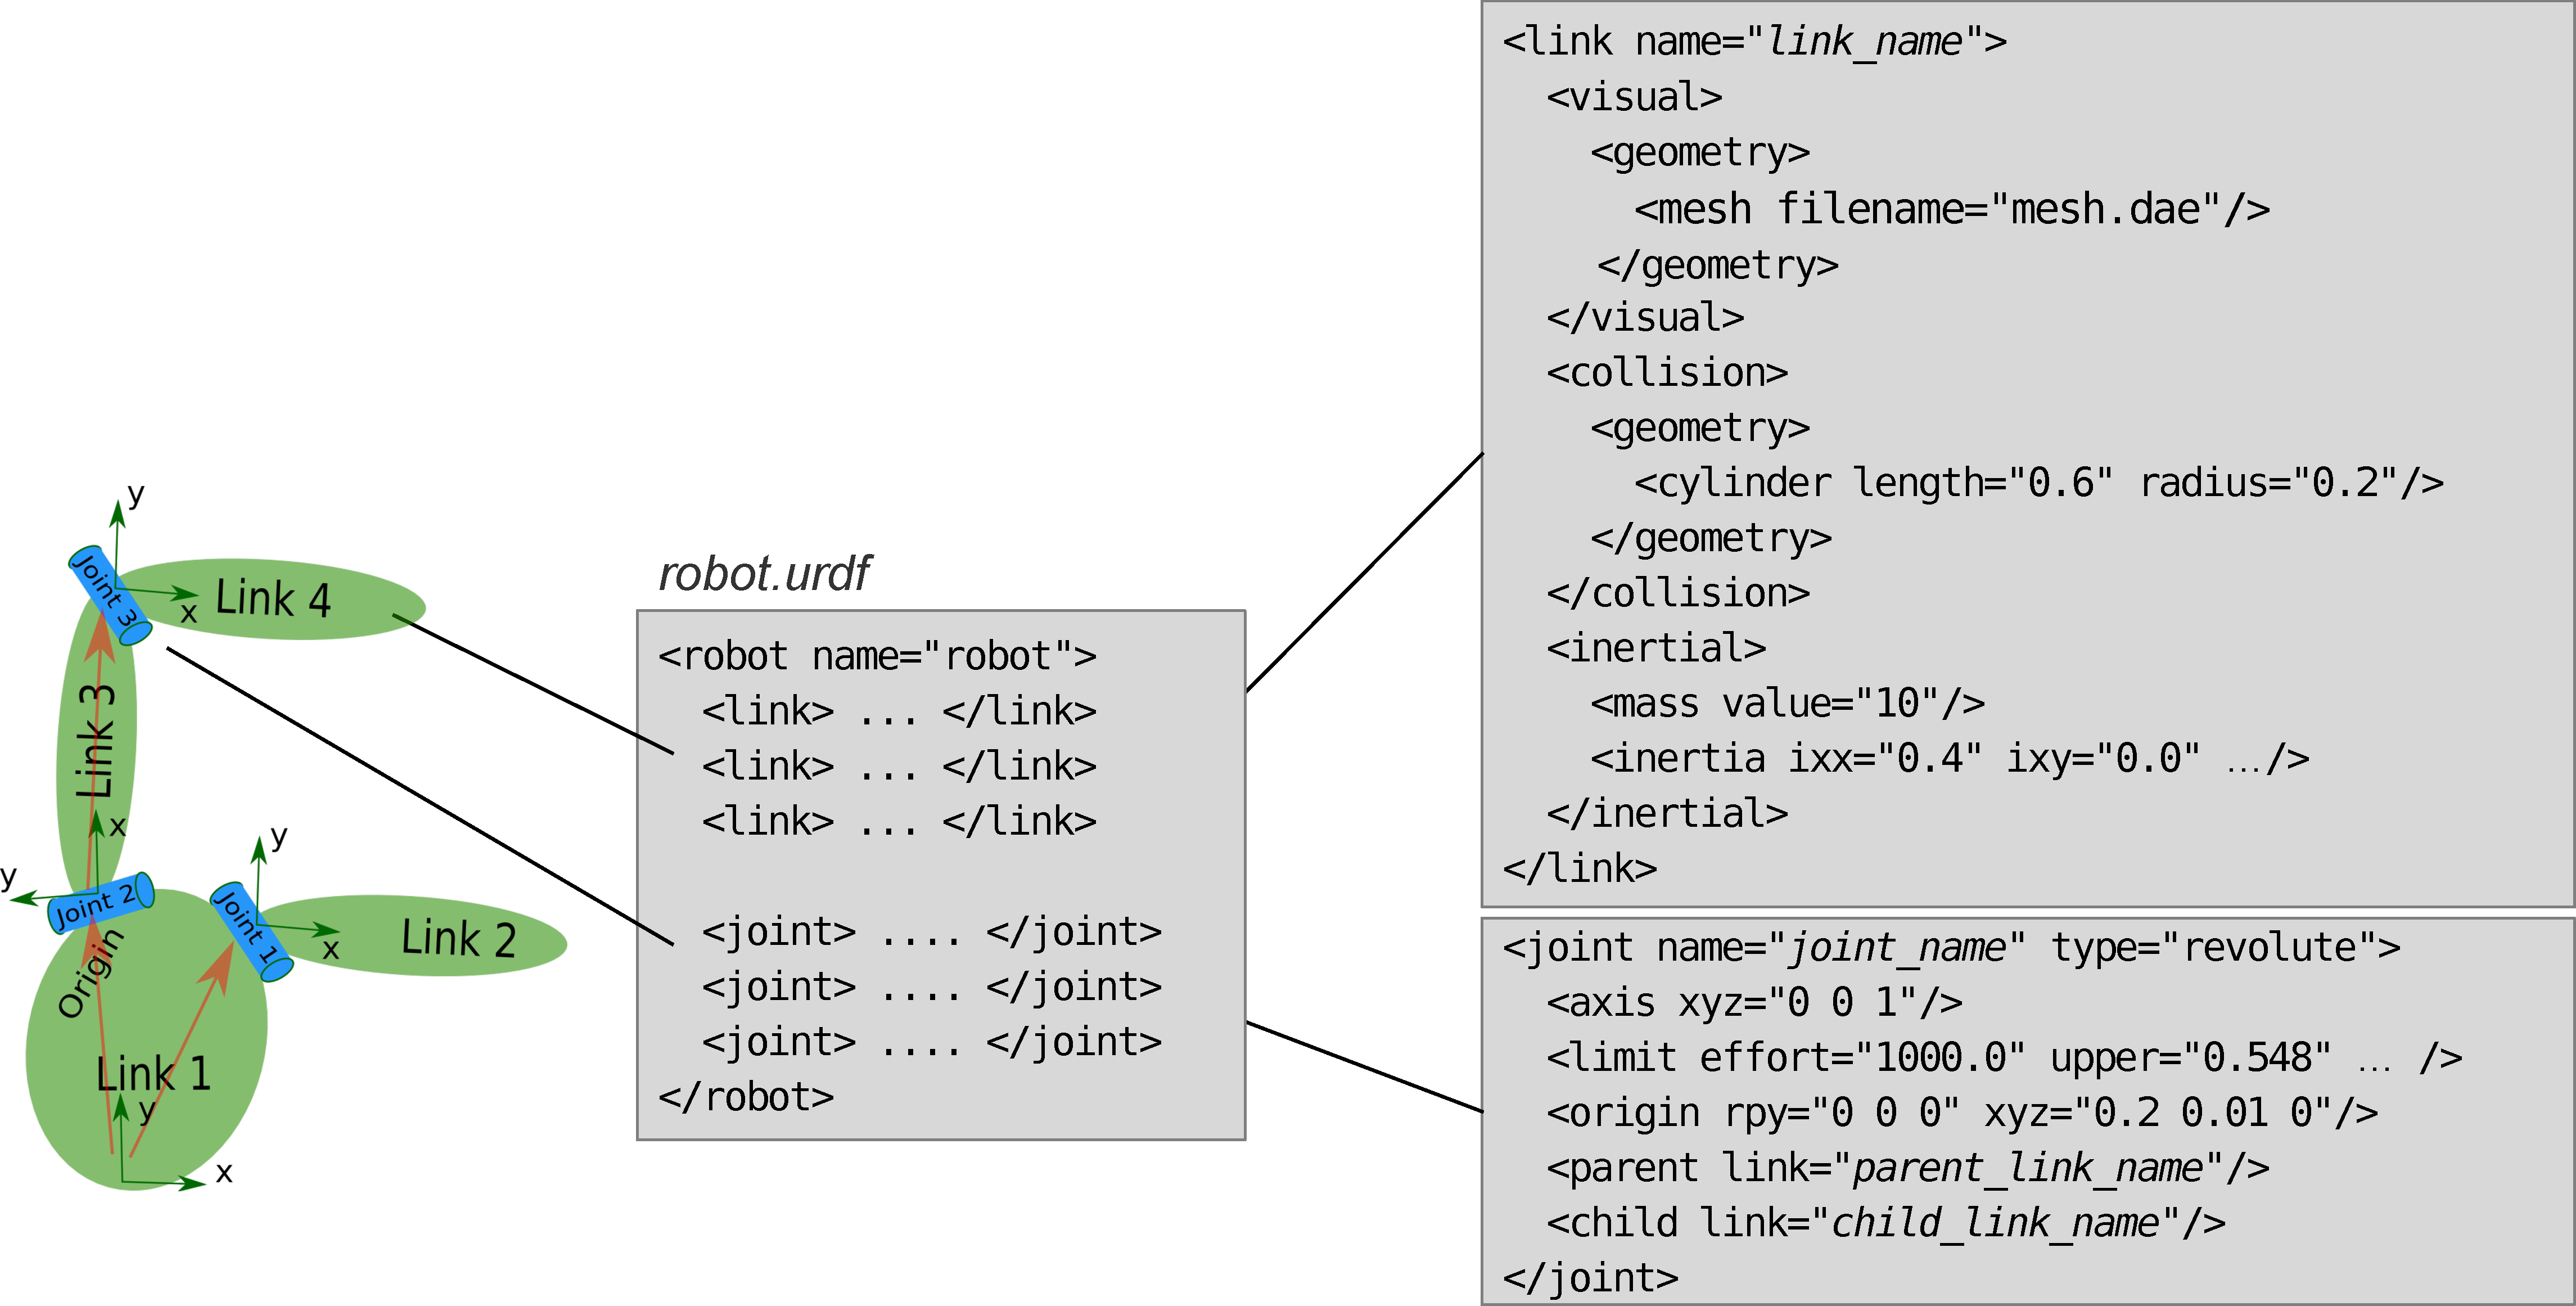
\includegraphics[width=0.8\columnwidth]{images/urdf_driagram.pdf}
	\end{figure}
    \note{https://wiki.ros.org/urdf/Tutorials}
    \note{https://articulatedrobotics.xyz/tutorials/ready-for-ros/urdf/}
    \note{Parámetro Collision: es utilizado para el cálculo de las colisiones físicas}
    \note{Parámetro Inertial: se utiliza para cálculos físicos, determina cómo responde el link a las fuerzas.}

\end{frame}

\begin{frame}[fragile]
    \frametitle{Unified Robot description Format (URDF)}
    
\footnotesize

\begin{columns}
\begin{column}{0.4\textwidth}
\begin{itemize}
\item La descripción del robot (URDF) está guardada en un servidor de parámetros como \lstinline[style=bash]{/robot_description}
\item Se puede visualizar el robot en RViz con el plugin \lstinline[style=bash]{RobotModel}
\end{itemize}
\end{column}
\begin{column}{0.6\textwidth}

\lstinline[style=bash]{control.launch}
\begin{lstlisting}[style=xml,basicstyle=\tiny]
...
<include file="$(find smb_description)/launch/load.launch">
<arg name="simulation"
value="$(arg simulation)"/>
<arg name="description_name" value="$(arg robot_description)"/>
<arg name="description_file" value="$(arg description_file)"/>
<arg name="wheel_joint_type" value="continuous"/>
<arg name="robot_namespace"
value="$(arg robot_namespace)"/>
</include>
...
\end{lstlisting}

\lstinline[style=bash]{load.launch}
\begin{lstlisting}[style=xml,basicstyle=\tiny]
...
<param name="$(arg description_name)" command="$(find xacro)/xacro
$(arg description_file)
wheel_joint_type:=$(arg wheel_joint_type)
simulation:=$(arg simulation)
robot_namespace:=$(arg robot_namespace)
lidar:=$(arg lidar)
description_name_xacro:=$(arg description_name)
publish_tf:=$(arg publish_tf)"/>
</launch>
...
\end{lstlisting}
	
\end{column}
\end{columns}

\end{frame}

\begin{frame}
    \frametitle{Simulation Description Format (SDF)}
    \footnotesize
   	\begin{columns}
    	\begin{column}{0.5\textwidth}
    		\begin{itemize}
    			\item Se define en un archivo XML para describir
	    		\begin{itemize}
    				\item Entorno (luces, gravedad, etc)
					\item Sensores
					\item Robots
    			\end{itemize}
			\item SDF es el formato estándar de Gazebo
			\item Gazebo convierte automáticamente URDF a SDF 
    		\end{itemize}
    	\end{column}
    	\begin{column}{0.5\textwidth}
    		\begin{figure}[!h]
    			\centering
				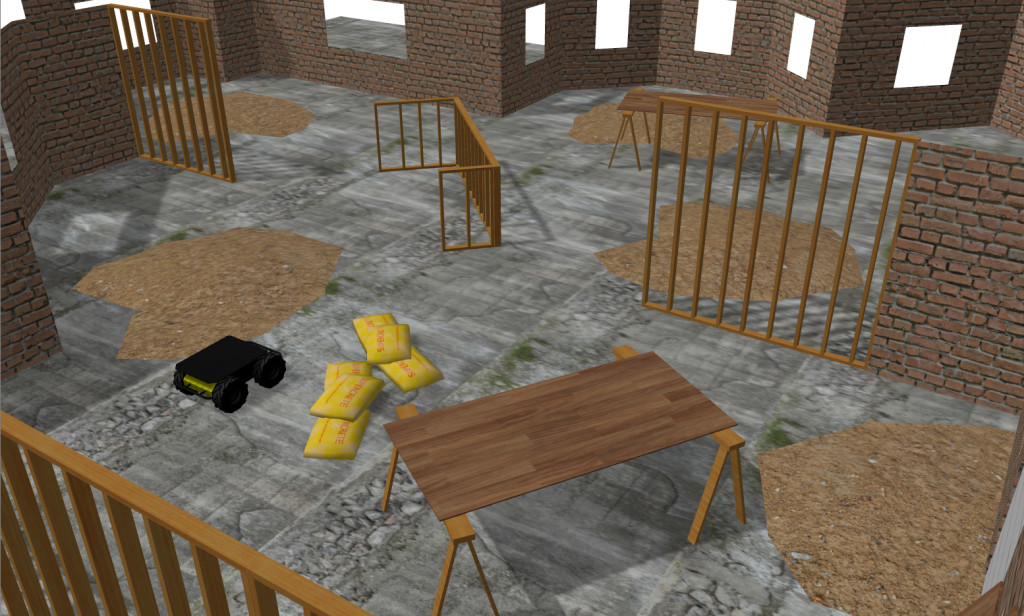
\includegraphics[width=\columnwidth]{images/sdf_gazebo.jpg}
    		\end{figure}
    	\end{column}
    \end{columns}
    
\end{frame}

\begin{frame}
    \frametitle{Estrategias de Debugging}
    
    \note{información extraida de https://youtu.be/ZQezxGadsqw}
    \begin{itemize}
        \item Compilar y correr código frecuentemente para atrapar errores tempranamente
        \item Entender los mensajes de error de compilación y ejecución
        \item Usar herramientas de análisis para verificar el flujo de los datos: \lstinline[style=bash]{ros2 node info}, \lstinline[style=bash]{ros2 topic echo}, \lstinline[style=bash]{ros2 wtf}, \lstinline[style=bash]{rqt\_graph}, etc.
        \item Visualizar y plotear los datos: \lstinline[style=bash]{RViz}, \lstinline[style=bash]{RQT Multiplot}, \lstinline[style=bash]{rqt_bag}, etc.
        \item Dividir el programa en pequeños pasos y verificar resultados intermedios (\lstinline[style=bash]{ROS_INFO}, \lstinline[style=bash]{ROS_DEBUG}, etc)
        \item Hacer el código robusto verificando argumentos de entrada y utilizar try-catch para atrapar excepciones
        \item Extender y optimizar el código solo cuando la versión básica este funcionando
        \item Si las cosas no tienen sentido, limpiar el workspace
        \item Debugguear con una IDE (utilizar breakpoints)
        \item Escribir Unit-tests y test de integración para encontrar regresiones
    \end{itemize}
    
\end{frame}

\begin{frame}
	\frametitle{Funcionalidades / Herramientas no cubiertas}
	
	\begin{itemize}
		\item Creación y uso de Servicios
		\item Creación de Mensajes customizados
		\item Uso de parámetros en un nodo
        \item \lstinline[style=bash]{rqt_bag}
		\item \lstinline[style=bash]{rqt_logger_level}
		\item \lstinline[style=bash]{rqt_console}
		\item \lstinline[style=bash]{rqt_graph}
		\item \lstinline[style=bash]{rqt_multiplot}
		\item \lstinline[style=bash]{rqt_image_view}
        \item \lstinline[style=bash]{foxglove} (Alternativa a \lstinline[style=bash]{RViz})
	\end{itemize}
	
\end{frame}


